\documentclass{article}
\usepackage{listings}
\usepackage{graphicx}
\usepackage{url}
\usepackage{hyperref}
\usepackage{amsmath}
\usepackage{xcolor}
\usepackage{subcaption}
\usepackage{float}
\graphicspath{ {./images/} }
\usepackage{gensymb}
\usepackage[english]{babel}
\usepackage[T1]{fontenc}
\usepackage[a4paper, top=2.5cm, bottom=2.5cm, left=3cm, right=3cm]{geometry}
\usepackage{listings}
\usepackage{inconsolata}
\pagenumbering{arabic}


\lstset{frame=single, showstringspaces=false, columns=fixed, basicstyle={\ttfamily}, commentstyle={\it}, numbers=left, tabsize=4}

\definecolor{codebackground}{RGB}{240, 248, 255} % Pale Blue
\definecolor{codecomment}{RGB}{106,153,85}
\definecolor{codekeyword}{RGB}{30,30,255}
\definecolor{codestring}{RGB}{163,21,21}
\definecolor{codenumber}{RGB}{100,100,100}

\lstdefinestyle{modernstyle}{
    backgroundcolor=\color{codebackground},
    commentstyle=\color{codecomment},
    keywordstyle=\color{codekeyword},
    numberstyle=\tiny\color{codenumber},
    stringstyle=\color{codestring},
    basicstyle=\ttfamily\footnotesize\color{black},
    breakatwhitespace=false,
    breaklines=true,
    captionpos=b,
    keepspaces=true,
    numbers=left,
    numbersep=5pt,
    showspaces=false,
    showstringspaces=false,
    showtabs=false,
    tabsize=4
}

\lstset{style=modernstyle}

\begin{document}
\title{Heat Simulation of a Single Heat Fin CPU Radiator}
\author{Pierre-Antoine LAMBRECHT/SENGER}
\date{\today}

\maketitle

\vspace{30pt} % Add 10 points of vertical space

\begin{figure}[H]
    \centering
    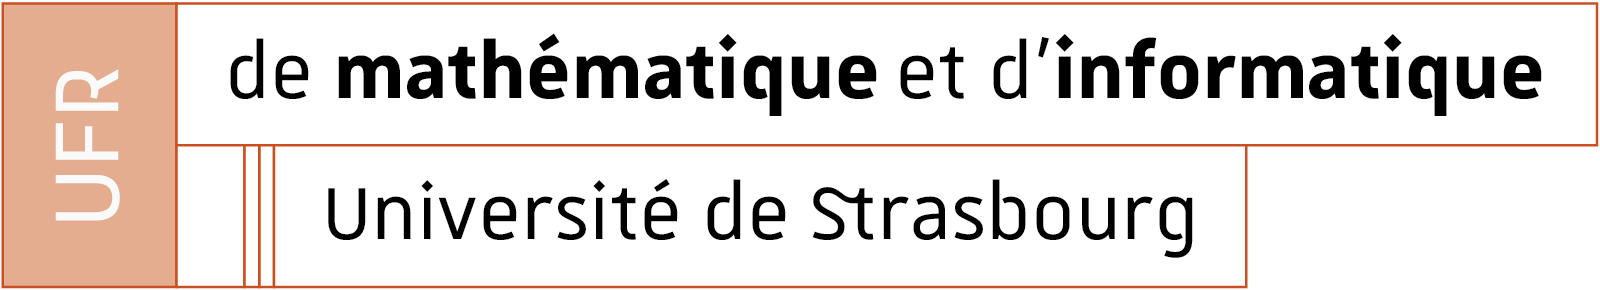
\includegraphics[width=1\linewidth]{image.png}   
\end{figure}

\vspace{30pt} % Add 10 points of vertical space

\tableofcontents
\newpage

\section{Compilation}
Place yourself in the root of the Project.  \\ 
Move or make a fresh build directory and move into it:
\begin{lstlisting}[language=bash]
mkdir build
cd build
\end{lstlisting}
Compile an executable :
\begin{lstlisting}[language=bash]
cmake --preset release ..
make
\end{lstlisting}

\section{Usage}

\subsection{Run a Simulation}
From the build directory do :
\begin{lstlisting}[language=bash]
./run <config_file>
\end{lstlisting}

Example:
\begin{lstlisting}[language=bash]
./run ../simul.cfg
\end{lstlisting} 

You can modify or make your own \textbf{configuration files} as long as it's \textbf{exactly} in the same \textbf{format}:
\begin{lstlisting}
Lx 40 Ly 4 Lz 50
Nx 10000
Phi 0.125
hc 0.0004
Te 20
rho 2700 
kappa 164
stationary 0
cycling 0
fan 1
cooling 0
TFinal 300
Nt 600
Mx 100 My 20 Mz 60
doPlots 1 do3D 1
solName test1 
\end{lstlisting}

\textbf{Note:} Writing into the files can take some time (with those parameters there are around $240,000 \times 600 = 144$ million small lines to write). 

\subsection{Visualization}

For 2D solutions, you can choose in the \texttt{simul.cfg} if you want to see the plots or not. Additionally, if you want to see more plots and testings, you can do:
\begin{lstlisting}[language=bash]
make test
\end{lstlisting}

Solutions are saved in \texttt{data}. \\
3D solutions can be visualized in a visualization software like \texttt{Paraview}.

\textbf{Note:} To do the plots, you will need the \texttt{pandas} library which can be installed using \href{https://pip.pypa.io/en/stable/}{pip} :
\begin{lstlisting}[language=bash]
pip install pandas
\end{lstlisting}
or using \href{https://www.anaconda.com/}{conda}/\href{https://github.com/mamba-org/mamba}{mamba}:
\begin{lstlisting}[language=bash]
conda install pandas
\end{lstlisting}
\begin{lstlisting}[language=bash]
mamba install -c conda-forge pandas
\end{lstlisting}


\textbf{Note:} If the data directory gets too big, you can simply delete it; the save functions know how to create one without crashing.

\section{Construction of the Project}

The details of the classes are given in a \texttt{Doxygen} documentation.  
You can open it from the root of the project with the browser of your choice:
\begin{lstlisting}[language=bash]
chromium html/index.html
\end{lstlisting}

\subsection{Tridiag}

\begin{lstlisting}[language=c++]
template <class T> class Tridiag {
public:
  Tridiag(std::size_t n = 1);
  Tridiag(const Tridiag &t);
  Tridiag(std::size_t n, T l, T d, T u);
  Tridiag &operator=(const Tridiag &t);
  ~Tridiag(){};

  //* Getters & Setters
  std::size_t size() const { return M_n; }
  T upper(int i) const { return M_upper[i]; }
  T diag(int i) const { return M_diag[i]; }
  T lower(int i) const { return M_lower[i]; }
  T &upper(int i) { return M_upper[i]; }
  T &diag(int i) { return M_diag[i]; }
  T &lower(int i) { return M_lower[i]; }
  T operator()(int i, int j) const;
  T &operator()(int i, int j);

  //* Arithmetic Operators & others methods
  Tridiag factorize() const;
  Tridiag &operator+=(const Tridiag &rhs);
  Tridiag &operator-=(const Tridiag &rhs);
  std::vector<T> operator*(const std::vector<T> &rhs) const;
  void clear(); ///< Clear the matrix vectors
  
  //* The following operators are defined outside the class :
  // Tridiag<T> operator+(const Tridiag<T> &lhs, const Tridiag<T> &rhs)
  // Tridiag<T> operator-(const Tridiag<T> &lhs, const Tridiag<T> &rhs
  // Tridiag<T> operator*(const double lhs, const Tridiag<T> &rhs)
  // Tridiag<T> operator*(const Tridiag<T> &lhs, const double rhs)
  // Tridiag<T> operator/(const Tridiag<T> &lhs, const double rhs)
  
  //* A method for solving LUx=b is defined outside the class:
  // void solveLU(std::vector<T> &x, const Tridiag<T> &LU, const std::vector<T>
  // &b)

  //* Ostream outsite of the class
  // template <class U>
  // friend std::ostream &operator<<(std::ostream &os, const Tridiag<U> &t);

private:
  std::size_t M_n;        ///< Dimention of the square matrix
  std::vector<T> M_upper; ///< Vector of the upper diagonal part
  std::vector<T> M_diag;  ///< Vector of the main diagonal part
  std::vector<T> M_lower; ///< Vector of the lower diagonal part
};
\end{lstlisting}

The problem is modeled using a \textbf{banded matrix}, so we started by making a \textbf{template class} \texttt{Tridiag} representing a tridiagonal matrix using 3 \texttt{std::vector<class T>} representing the \textbf{upper}, \textbf{lower}, and \textbf{main diagonal} of the matrix. \\ 

The \texttt{Tridiag} class has well-defined accessors in writing/reading as well as an ostream operator. It also has some arithmetic operators defined left and right to make the code more readable. It could be improved by adding a matrix-vector multiplication, which can be useful in solving dynamic systems (I'll do it if I have the time and don't forget). \\

To efficiently solve a linear system, the class can factorize a \texttt{Tridiag} object A using an LU factorization: $A=LU$ where,\\ $L$ is bidiagonal \textbf{lower} (with ones on the main diagonal like in every LU factorization), \\
$U$ is bidiagonal \textbf{superior}.  \\ 

Since there is no point storing the ones of $L$, the LU factorization is stored in a \textbf{single Tridiag} object where, \\ 
\texttt{Tridiag.lower} represent the lower diagonal of $L$,  \\
\texttt{Tridiag.diag} represent the main diagonal of $U$,  \\
\texttt{Tridiag.upper} represent the upper diagonal of $U$.  \\

\[
L =
\begin{pmatrix}
    1 & 0&\cdots & \cdots & 0 \\
    l_{21} & 1 & \ddots& & \vdots \\
    0 & l_{32} & 1 &\ddots & \vdots \\
    \vdots &\ddots & \ddots & \ddots & 0\\
    0 & \cdots & 0 & l_{n,n-1} & 1
\end{pmatrix}
\quad
U =
\begin{pmatrix}
    u_{11} & u_{12} & \cdots & \cdots & 0 \\
    0 & u_{22} & u_{23} &  & \vdots\\
    \vdots & \ddots & u_{33} & \ddots & \vdots\\
    \vdots &  &  \ddots & \ddots & u_{n-1, n}\\
    0& \cdots& \cdots&0 & u_{nn}
\end{pmatrix}
\]

\[
LU =
\begin{pmatrix}
    u_{11} & u_{12} & 0 & \cdots  & 0 \\
    l_{21} & u_{22} & u_{23} &  \ddots & \vdots \\
     0& l_{32} & u_{33} & \ddots & 0 \\
     \vdots&\ddots & \ddots & \ddots & u_{n-1,n}  \\
     0 & \cdots & 0 & l_{n, n-1} & u_{nn}
\end{pmatrix}
\]



The file \texttt{tridiag.hpp} also contains a function \texttt{solveLU} which take a LU matrix as described above and solve a \textbf{LUx=b} system with a time complexity in $O(n)$.

\subsection{Model}
\begin{lstlisting}[language=c++]
using dvector = std::vector<double>;

class Model {
public:
  Model(std::size_t Nx, double x0, double xend);
  Model(const Model &m);
  Model &operator=(const Model &m);
  virtual ~Model(){};

  virtual void setLU() = 0;
  virtual void setB(dvector, double, std::size_t, double) = 0;
  virtual void setU0(double u0);
  virtual void setXend(double d); ///< End of discretization
  virtual void setMesh(Mesh3D &mesh) { M_mesh = &mesh; }
  void setDt(double d); ///< Time step value

  virtual double b(std::size_t i) const;
  virtual double solveExact(double);
  std::size_t Nx() const;        ///< Numbers of space steps
  double x0() const;             ///< Start of discretization
  double xend() const;           ///< End of discretization
  double x(std::size_t i) const; ///< Value in discretization
  double u(std::size_t i) const; ///< Value in vector solution
  double dx() const;             ///< Space step value
  Tridiag<double> S();           ///< Matrix of the model
  dvector &u();                  ///< Returns whole solution 
  dvector &b();                  ///< Returns whole RHS vector

protected:
  std::size_t M_Nx;    ///< Number of space steps
  double M_x0;         ///< Start of the discretization
  double M_xend;       ///< End of the discretization
  dvector M_x;         ///< Vector of the discretization
  dvector M_u;         ///< Vector of initial contition
  Tridiag<double> M_S; ///< Matrix of the model
  dvector M_b;         ///< RHS of the model
  double M_dt;         ///< Time step
  Mesh3D *M_mesh;      ///< Pointer on a mesh for 3d visualization
};
\end{lstlisting}
We then created a \textbf{abstract base class} \texttt{Model} to modelize the problem to solve.   \\

This base class is supposed to put the foundation of what any model should have and should implement. It's an \textbf{abstract class} so if we want to solve other problems with similar methods we can just add new models and have a solver with a pointer to a base \texttt{Model}. \\

The most important member attributes are \textbf{Nx}, the number of space steps we're going to use in our discretization of the problem and will translate into the size of the matrix of the method \textbf{S} and the right-hand side vector \textbf{b} of the linear system modeling the problem. \\

This is why \texttt{Model} has 2 pure virtual methods \texttt{setLU} and \texttt{setB} to ensure all derived classes implement correctly the \textbf{tridiagonal matrix of the method} (and factorize it in its LU form right away) as well as \textbf{b}, the \textbf{RHS} of the system $Ax=b$.\\
Note that in order to be able to solve dynamic systems \texttt{setB} takes in argument the vector of current solution, the time (in case we are in a cycling model), the number of space steps \texttt{Nt} as well as the final time \texttt{tf}.\\

In order to make a 3D visualization of the solutions a model can also have a pointer to a \textbf{class} \texttt{Mesh3D} (I don't think we need more than 3D representation so there is no base class for it).

\subsection{HeatFin}
\begin{lstlisting}[language=c++]
class HeatFin : public Model {
public:
  HeatFin(double nx, double rho, double c, double k, double Te, double phi,
          double hc, double Lx, double Ly, double Lz);
  HeatFin(const HeatFin &f);
  HeatFin &operator=(const HeatFin &f);
  ~HeatFin() {}

  void setLU() override;
  void setB(dvector u, double t, std::size_t nt, double tf) override;
  void fanON();
  void fanOFF();
  void fluxON();
  void fluxOFF();
  void CoolingON();
  void CoolingOFF();
  void setHc(double power);    ///< Fan power
  void setCooler(double temp); ///< Cooling power
  void setPhi(double d);       ///< Heat flux power
  void setLx(double d);        ///< Same as setXend() from base class
  void setCycling(bool b);     ///< Cycling status ON or OFF
  void setStationnary(bool b); ///< Dynamic or stationnary model

  void interpolate(dvector &U);
  void interpolate(std::vector<dvector> &T, std::size_t Nt,
                   const std::string solName);

  void saveStaticInterpolation(const std::string filename);

  double solveExact(double x) override;
  bool flux() const;    ///< Current status of the flux
  bool cooling() const; ///< Current status of the cooling
  double p() const;     ///< Perimeter
  double s() const;     ///< Surface
  double hc() const;    ///< Fan power

protected:
  double M_rho; ///< Density
  double M_C;   ///< Heat at constant pressure
  double M_k;   ///< Thermal conductivity
  double M_Te;  ///< External Temperature
  double M_phi; ///< Heat flux power
  double M_hc;  ///< Heat surfacic transfer coefficient
  double M_Ly;  ///< Size of the fin on the y-axis
  double M_Lz;  ///< Size of the fin on the z-axis
  ///< M_Lx = Model::M_xend
  double M_cooler;      ///< Cooling power effect (so <0)
  bool M_flux;          ///< Heat flux status
  bool M_cooling;       ///< Cooling status, why did I do this?
  bool M_cyclingStatus; ///< Status of the heat flux
  bool M_stationnary;   ///< Stationnary or Dynamic model
  dvector M_staticInterpolation;
  // Cooling need to be changed to accuratly describe what happens IRL
};
\end{lstlisting}

For our particular problem, we created a \textbf{derived class} of \texttt{Model} called \texttt{HeatFin} which fully describes the setups with the dimensions of the fin, the physical conditions, if we solve a stationary model or dynamic, with constant heat flux or cycling etc.\\

The \texttt{setLU} and \texttt{setB} methods are correctly overridden using the equations given in the subject. For the dynamic system,\\
\begin{equation}\label{eq:heat_equation}
\rho C_p \frac{T_{i}^{n+1} - T_{i}^{n}}{\Delta t} - \kappa \frac{T_{i-1}^{n+1} - 2T_{i}^{n+1} + T_{i+1}^{n+1}}{\Delta x^2} + \frac{h_c p}{S} (T_i^{n+1} - T_e) = 0 
\end{equation}
gives us,
\begin{equation}\label{eq:matrix_equation}
\left(\frac{\rho C_p}{\Delta t} + \frac{h_c p}{S}\right) I + \frac{\kappa}{\Delta x^2} A = B T^n + B'
\end{equation}

with,
\[
I = 
\begin{pmatrix}
    0 & 0 & \cdots & \cdots & 0 \\
    0 & 1 & \ddots &  & \vdots \\
    \vdots & \ddots & \ddots & \ddots & \vdots \\
    \vdots &  & \ddots & 1 & 0 \\
    0 & \cdots & \cdots & 0 & 0
\end{pmatrix}
\quad
A = 
\begin{pmatrix}
    \Delta x & -\Delta x & 0    & \cdots & 0  \\
    -1      & 2         & -1     & \ddots & \vdots  \\
    0       & \ddots    & \ddots & \ddots & 0 \\
    \vdots  &    \ddots  & -1 & 2 & -1 \\
    0         & \cdots  &    0    & -\Delta x& \Delta x 
\end{pmatrix}
\]
\[
B = 
\begin{pmatrix}
    \Phi_p \\ \frac{\rho C_p}{\Delta t} \\ \vdots \\ 0
\end{pmatrix}
\quad
B' = 
\begin{pmatrix}
    0 \\ \frac{T_e h_c p}{S} \\ \vdots \\ 0
\end{pmatrix}
\]
\begin{itemize}
\item $\rho$ : density 
\item $C_p$ : specific heat at constant pressure 
\item $\kappa$ : thermal conductivity
\item $h_c$ : surface heat transfer coefficient
\item $S = L_y L_z$ : cross-sectional area
\item $p = 2(L_y + L_y)$ : cross-sectional perimeter
\item $\Phi_p$ : heat flux power 
\end{itemize}


This class also has the \texttt{interpolate} (static and dynamic) methods which in the case of the static model take the vector of \textbf{solution} in argument to calculate the values for the 3D visualization and can be saved with another method \texttt{saveStaticInterpolation}.\\

In the case of the dynamic model, \texttt{interpolate} takes the vector of vectors containing all the \textbf{solutions in time} (one for each time step \texttt{Nt}) as well as the time step \texttt{Nt}, the \textbf{name} of the solution used in the saving of the file (the dynamic interpolation re-uses the \texttt{saveStaticInterpolation} for each time step). It would save disk space to directly write the interpolation data into the files instead of storing them in a vector but it's also less readable and also takes more time somehow (maybe because the file is open and adds charges on the CPU?) \\


\subsection{SolverTime}
\begin{lstlisting}[language=c++]
using dvector = std::vector<double>;

class SolverTime {
public:
  SolverTime(std::size_t Nt = 0, double tf = 1);
  SolverTime(const SolverTime &s);
  SolverTime &operator=(const SolverTime &s);
  ~SolverTime();

  double dt() const; ///< Get the time step value

  void setTfinal(double t);   ///< Sets the final time value
  void setNt(std::size_t nt); ///< Sets the number of time steps
  void setModel(Model &m);    ///< Sets a pointer to a Model
  void solveStatic();         ///< Solves a stationary Model
  void solve();               ///< Solves a dynamic Model 
  void solve(double tFinal);

  std::vector<dvector> &T() { return M_T; } 
  dvector &U() { return M_U; }              
  void saveStatic(const std::string filename, const bool do_plot = false);
  void saveAtTimes(const std::string filename, dvector times,
                   const bool do_plot = false);
  template <typename... Args>
  void saveAtTimes(const std::string &filename, bool do_plot, Args... args);
  void saveAtPoints(const std::string filename,
                    const std::vector<double> points,
                    const bool do_plot = false);
  template <typename... Args>
  void saveAtPoints(const std::string &filename, bool do_plot, Args... args);

private:
  std::size_t M_Nt;         ///< Number of time steps
  double M_Tfinal;          ///< Final time
  std::vector<dvector> M_T; ///< Solutions in time
  dvector M_xt;             ///< Time discretization
  Model *M_model;           ///< Pointer to a model to solve
};
\end{lstlisting}
Finally, to solve the problem, we created a \textbf{class} \texttt{SolverTime} which is defined by the number of time steps \texttt{Nt}, the final time \texttt{Tfinal}, the vector of time discretization \texttt{xt}, the vector of all solutions in time \texttt{T}, and a pointer to a base class \texttt{Model} to solve.\\

As most of the information is stored in the model, \texttt{SolverTime} doesn't require a lot of methods. \\
The main ones are, of course, the solve methods with \texttt{solveStatic} which solve a \textbf{stationary} model and \texttt{solve} which solves a \textbf{dynamic} model and will use the final time set in the \texttt{SolverTime} object or can take a final time as an argument. \\

The class also has multiple save methods to \textbf{save and plot} the 2D results (which took me a lot of time to implement properly...) \\
Each saves methods has a boolean argument to do the plot or only the data saving (which are stored in \texttt{data/2d}).\\ 

\texttt{saveStatic} saves the stationary model with the \textbf{exact solution} next to it for comparison.\\ 

\texttt{saveAtTimes} saves at a particular time given in \textbf{seconds} by a vector, or an arbitrary number of times (variadic function) which is converted to the (approximated) index in the time discretization. Then plots all of them in one figure.\\  

\texttt{saveAtPoints} works similarly but with \textbf{point.s} on the physical model instead of \textbf{time.s}. \\

All the save methods "simply" look for the correct solutions to save; they don't require redoing the computation. \\
Each save method has a dedicated python plotting file stored in the \texttt{plotting} directory which contains all the necessary instructions to realize the plots using \texttt{pandas} and \texttt{matplotlib}. \\

This class could be improved by specifying the particular times we are interested in before solving the model so we could only store those instead of all the solutions in times thus saving a lot of spaces on the disk.

\subsection{Mesh}
\begin{lstlisting}[language=c++]
class Mesh3D {
public:
  Mesh3D(double Lx, double Ly, double Lz, int x, int y, int z)
      : M_Lxyz(3), M_Mxyz(3), M_x(x + 1), M_y(y + 1), M_z(z + 1) {
    setLxyz(Lx, Ly, Lz);
    setMxyz(x, y, z);

    for (std::size_t i = 0; i <= Mx(); ++i)
      M_x[i] = i * dx();
    for (std::size_t i = 0; i <= My(); ++i)
      M_y[i] = i * dy();
    for (std::size_t i = 0; i <= Mz(); ++i)
      M_z[i] = i * dz();
  }
  double Lxyz(int i) const { return M_Lxyz[i]; }
  double &Lxyz(int i) { return M_Lxyz[i]; }
  std::size_t Mxyz(int i) const { return M_Mxyz[i]; }
  std::size_t &Mxyz(int i) { return M_Mxyz[i]; }
  double Lx() const { return M_Lxyz[0]; } 
  double Ly() const { return M_Lxyz[1]; } 
  double Lz() const { return M_Lxyz[2]; } 
  double x(int i) const { return M_x[i]; }
  double y(int i) const { return M_y[i]; }
  double z(int i) const { return M_z[i]; }
  double &x(int i) { return M_x[i]; }
  double &y(int i) { return M_y[i]; }
  double &z(int i) { return M_z[i]; }
  std::size_t Mx() const { return M_Mxyz[0]; } 
  std::size_t My() const { return M_Mxyz[1]; } 
  std::size_t Mz() const { return M_Mxyz[2]; } 
  std::size_t &Mx() { return M_Mxyz[0]; }      
  std::size_t &My() { return M_Mxyz[1]; }     
  std::size_t &Mz() { return M_Mxyz[2]; }     
  void setLxyz(double x, double y, double z) {
    M_Lxyz[0] = x;
    M_Lxyz[1] = y;
    M_Lxyz[z] = z;
  }
  void setMxyz(int x, int y, int z) {
    M_Mxyz[0] = x;
    M_Mxyz[1] = y;
    M_Mxyz[2] = z;
  }
  double dx() const { return Lx() / Mx(); }
  double dy() const { return Ly() / My(); }
  double dz() const { return Lz() / Mz(); }
  dvector x_ijk(int i, int j, int k) const {
    dvector res(3);
    res[0] = x(i);
    res[1] = y(j);
    res[2] = z(k);
    return res;
  }

private:
  dvector M_Lxyz;    ///< Dimention of the model to mesh
  sizeVector M_Mxyz; ///< Number of steps in each dimention
  dvector M_x;       ///< Discretization in the x-axis
  dvector M_y;       ///< Discretization in the y-axis
  dvector M_z;       ///< Discretization in the z-axis
};
\end{lstlisting}
I made the \textbf{class} \texttt{Mesh} mechanically while reading the subject and by doing so implementing a lot of member attributes, and methods which are in the end not needed for our problem. I chose to keep them nonetheless in case we need it for future models. If not they can be removed to optimize memory usage. 

\subsection{SimulParam}
\begin{lstlisting}[language=c++]
struct SimulParam {
  // This contructor exist solely to silence -Weffc++ ...
  SimulParam()
      : Lx(), Ly(), Lz(), Phi(), hc(), Te(), tFinal(), rho(), kappa(), Nx(),
        Nt(), Mx(), My(), Mz(), stationary(), cycling(), doPlots(), fan(),
        cooling(), do3D(), solName() {}

  double Lx, Ly, Lz, Phi, hc, Te, tFinal, rho, kappa;
  std::size_t Nx, Nt, Mx, My, Mz;
  bool stationary, cycling, doPlots, fan, cooling, do3D;
  std::string solName;

  friend std::ostream &operator<<(std::ostream &os, const SimulParam &params);
  friend std::istream &operator>>(std::istream &is, SimulParam &params);
};
\end{lstlisting}
In order to avoid recompiling for each new simulation, a \texttt{SimulParam} struct is used to read and store the \textbf{configuration} of the simulation in an object given by the user in the configuration file. (This could maybe be done using a \texttt{std::map} instead)

\section{Results}
There is an infinity possible simulations, but it will also take an infinity amount of time and resources so let's look at only some of them.

\subsection{Convergence of the dynamic model}
We want to confirm that the dynamic model converges to the stationary model. We're going to compare the results of both simulations using same physical and geometrical parameters as in the subject :

\begin{figure}[H]
    \centering
    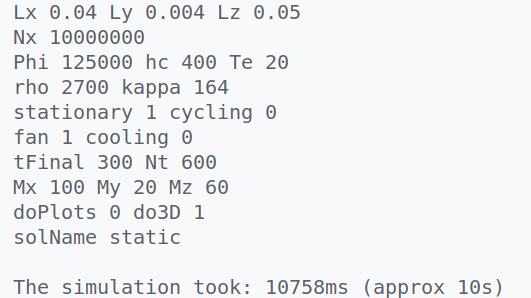
\includegraphics[width=.5\linewidth]{params.png}
    \caption{Parameters}
    \label{fig:enter-labe}
\end{figure}

\begin{figure}[H]
\begin{subfigure}{.5\textwidth}
  \centering
  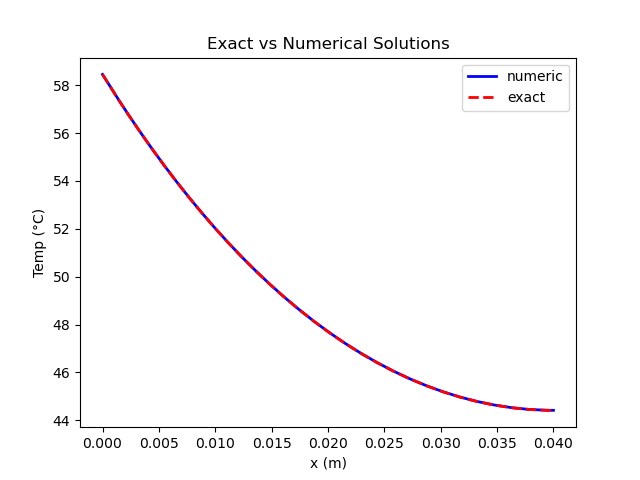
\includegraphics[width=1.1\linewidth]{images/static_graph.png}
  \caption{Stationary}
  \label{fig:sfig1}
\end{subfigure}
\begin{subfigure}{.5\textwidth}
  \centering
  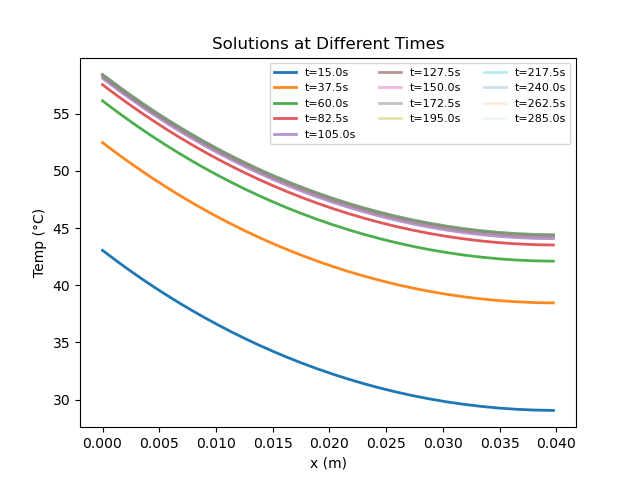
\includegraphics[width=1.1\linewidth]{images/dyna_graph.png}
  \caption{Dynamic}
\end{subfigure}
\caption{Stationary vs Dynamic }
\label{fig:fig}
\end{figure}

As we can see the dynamic model indeed converges to the stationary one in about 200s . (The stationary solution is confirmed by the exact solution available for this model). 

We can take a look at the 3d visualization for both cases :

\begin{figure}[H]
\begin{subfigure}{.5\textwidth}
  \centering
  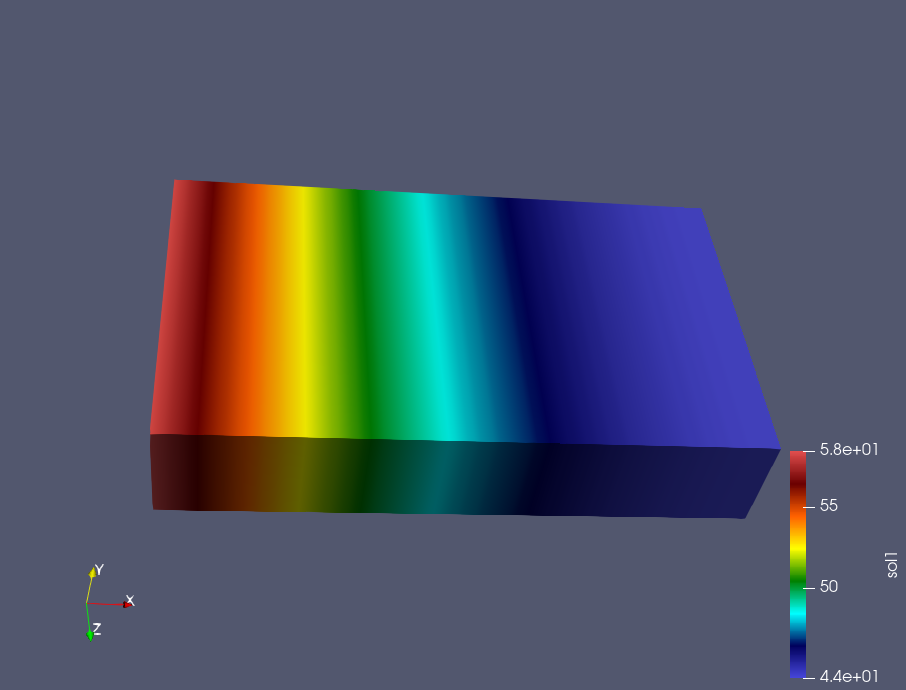
\includegraphics[width=1\linewidth]{images/static_3d.png}
  \caption{Stationary}
  \label{fig:sfig1}
\end{subfigure}
\begin{subfigure}{.5\textwidth}
  \centering
  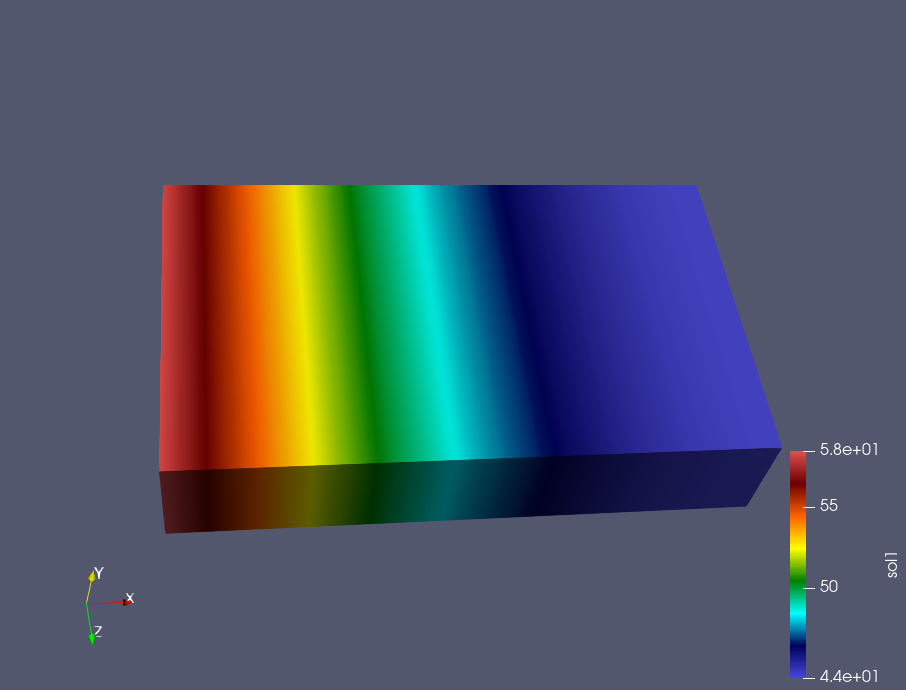
\includegraphics[width=1\linewidth]{images/dyna_200s.png}
  \caption{Dynamic after 200s}
\end{subfigure}
\caption{Stationary vs Dynamic}
\label{fig:fig}
\end{figure}


\subsection{Effect of Fin Length}
We're going to look at the difference between a 40mm length fin versus a 80mm one, the other physical parameters stays the same. \\

\begin{figure}[H]
\begin{subfigure}{.5\textwidth}
  \centering
  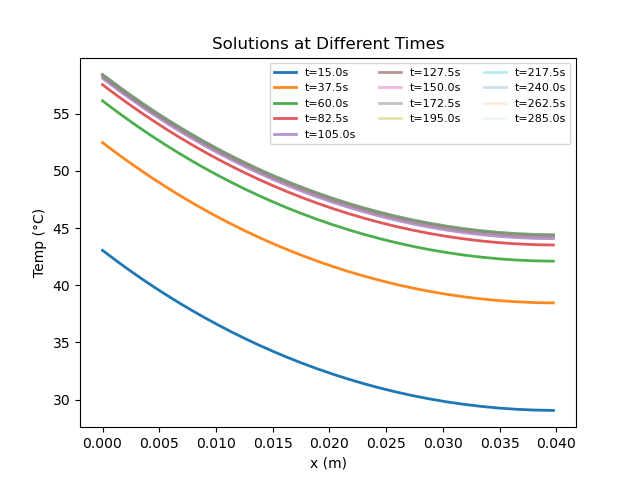
\includegraphics[width=1.1\linewidth]{images/graph40mm_standard.png}
  \caption{$L_x=40mm$}
  \label{fig:sfig1}
\end{subfigure}
\begin{subfigure}{.5\textwidth}
  \centering
  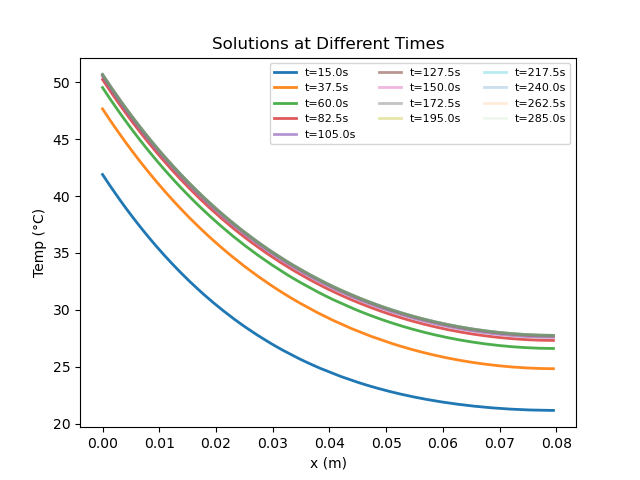
\includegraphics[width=1.1\linewidth]{images/graph80mm.png}
  \caption{$L_x=80mm$}
\end{subfigure}
\caption{$L_x=40mm$ vs $L_x=80mm$  }
\label{fig:fig}
\end{figure}


\begin{figure}[H]
\begin{subfigure}{.5\textwidth}
  \centering
  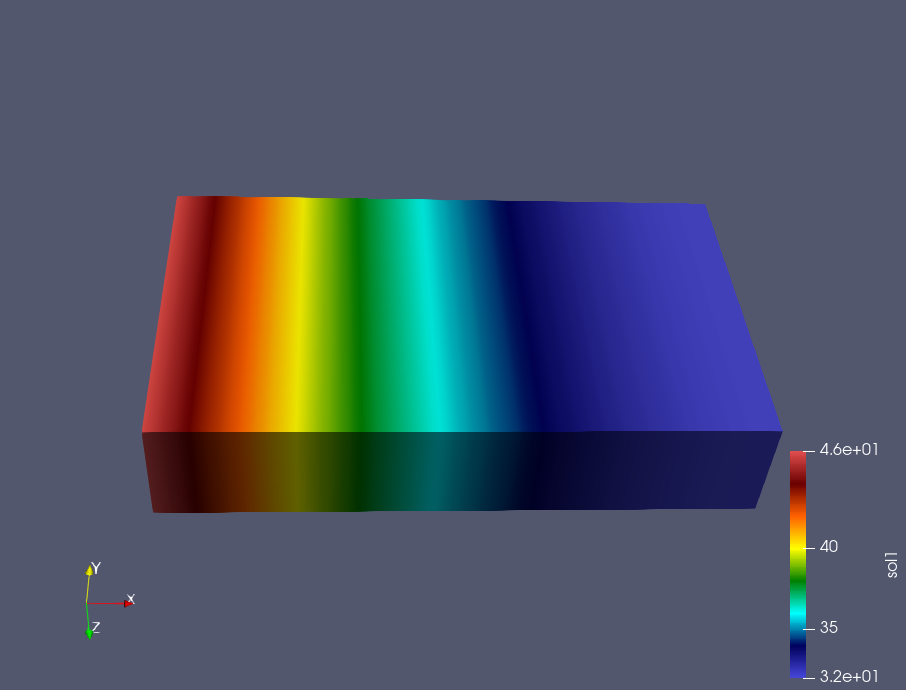
\includegraphics[width=1\linewidth]{images/standard40_40s.png}
  \caption{$L_x=40mm$}
  \label{fig:sfig1}
\end{subfigure}
\begin{subfigure}{.5\textwidth}
  \centering
  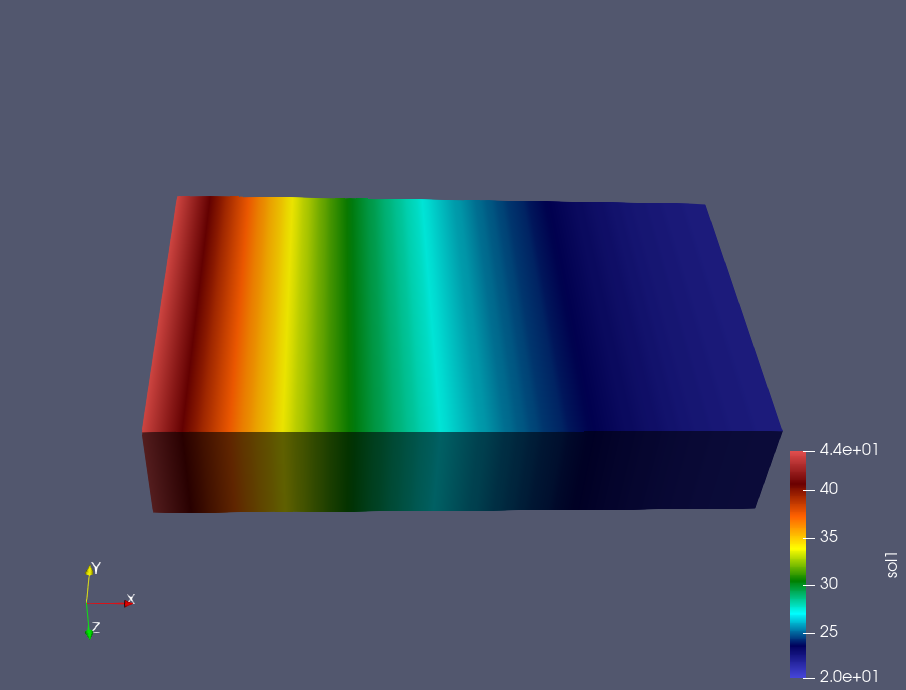
\includegraphics[width=1\linewidth]{images/standard80_40s.png}
  \caption{$L_x=80mm$}
\end{subfigure}
\caption{$L_x=40mm$ vs $L_x=80mm$ after 20s }
\label{fig:fig}
\end{figure}

\begin{figure}[H]
\begin{subfigure}{.5\textwidth}
  \centering
  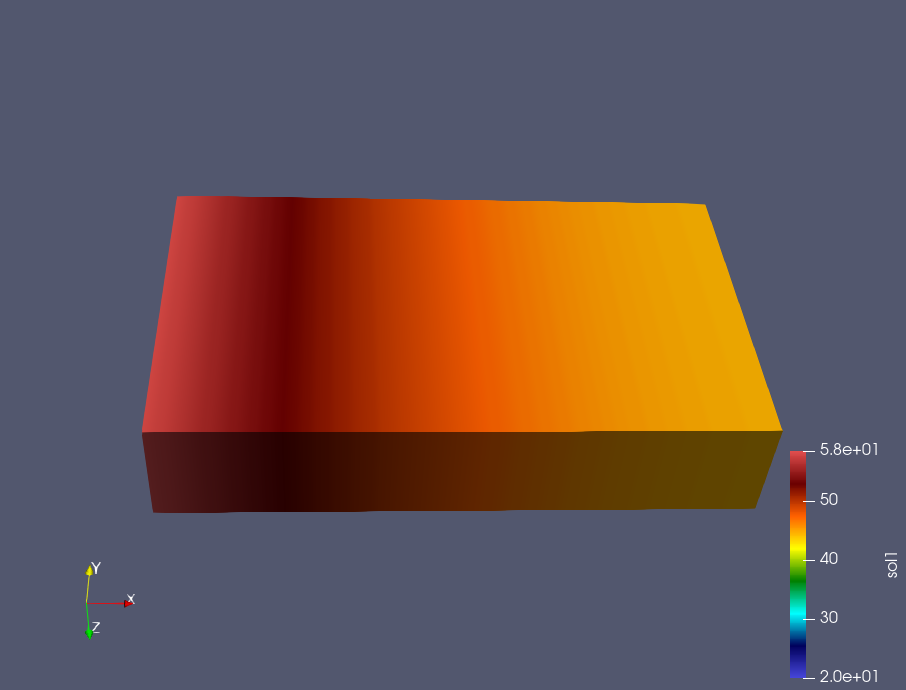
\includegraphics[width=1\linewidth]{images/standart40_350s.png}
  \caption{$L_x=40mm$}
  \label{fig:sfig1}
\end{subfigure}
\begin{subfigure}{.5\textwidth}
  \centering
  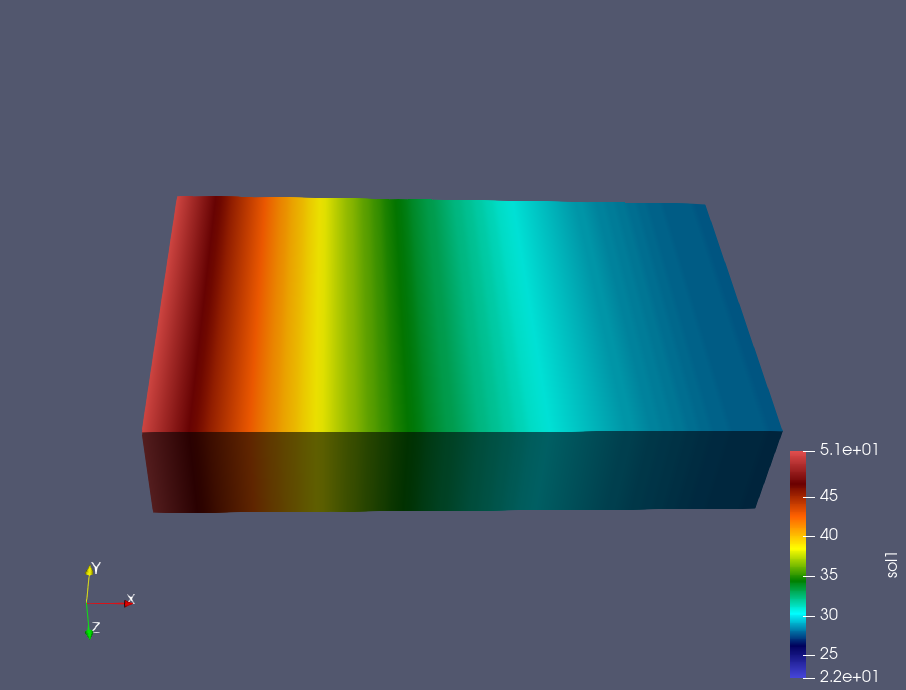
\includegraphics[width=1\linewidth]{images/standard80_400s.png}
  \caption{$L_x=80mm$}
  \label{fig:sfig2}
\end{subfigure}
\caption{$L_x=40mm$ vs $L_x=80mm$ after 200s}
\label{fig:fig}
\end{figure}

When it comes to radiator heat fin, size does matter. Already after 20 seconds, differences become apparent, especially at both ends.

After approximately 200 seconds, both models appear stable, with a noticeable temperature difference between them. Even at the point of contact, the 80mm fin is approximately 5$\degree$C cooler. This suggests good thermal conductivity for the material.

However, it's worth noting that the 40mm model doesn't exceed 60$\degree$C, which might be acceptable depending on the specific situation and potential temperature variations with other parameters.

\subsection{Cycling Heat Flux Scenarios}
Let's now look at a configuration with the fan ON and a cycling heat flux (30s ON 30s OFF) on a 40mm heat fin.\\

\begin{figure}[H]
\begin{subfigure}{.5\textwidth}
  \centering
  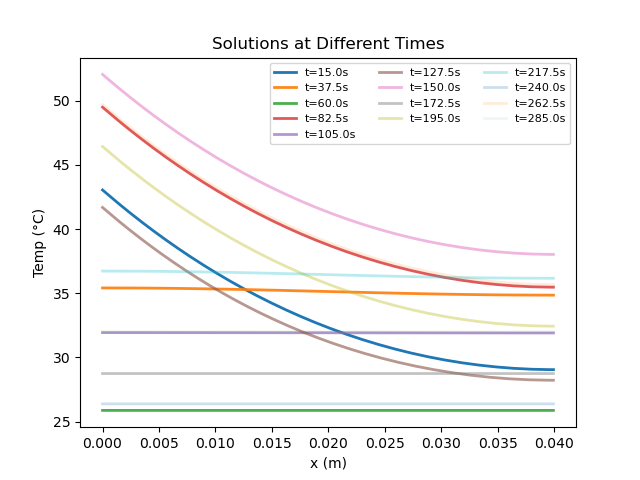
\includegraphics[width=1.1\linewidth]{images/cycl1.png}
  \caption{}
  \label{fig:sfig1}
\end{subfigure}
\begin{subfigure}{.5\textwidth}
  \centering
  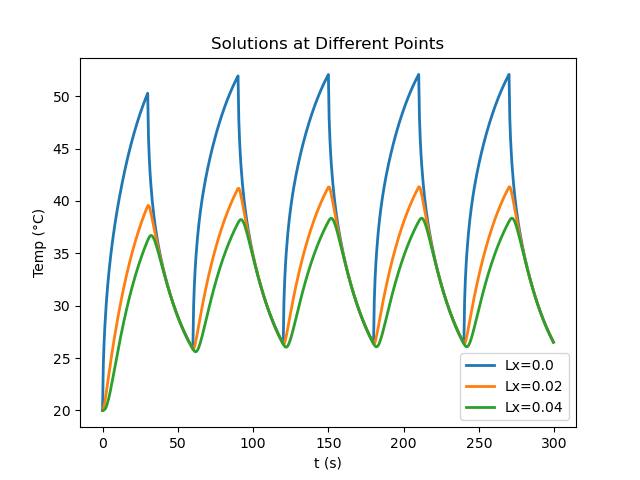
\includegraphics[width=1.1\linewidth]{images/cycl2.png}
  \caption{}
\end{subfigure}
\caption{Cycling heat flux}
\label{fig:fig}
\end{figure}

As we can see, the temperature in the fin rapidly decreases to approximately 26$\degree$C when the heat flux is turned off, even at the point of contact with the CPU. This reinforces our hypothesis regarding the thermal conductivity of the material. (This is also a very satisfying 3d simulation to watch). \\ 

\textbf{Note} that some solution appears almost constant which is not too surprising considering we are in a cycling model.

\subsection{Impact of Fan Operation}
What would happens in the case of a fan malfunction ? \\

\begin{figure}[H]
\begin{subfigure}{.5\textwidth}
  \centering
  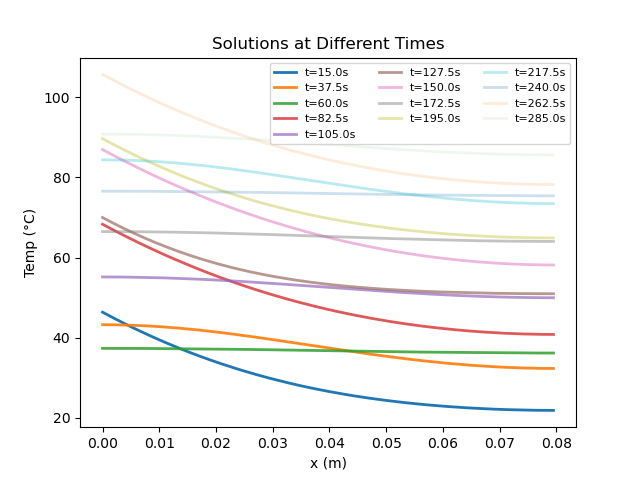
\includegraphics[width=1\linewidth]{images/noFan.png}
  \caption{}
  \label{fig:sfig1}
\end{subfigure}
\begin{subfigure}{.5\textwidth}
  \centering
  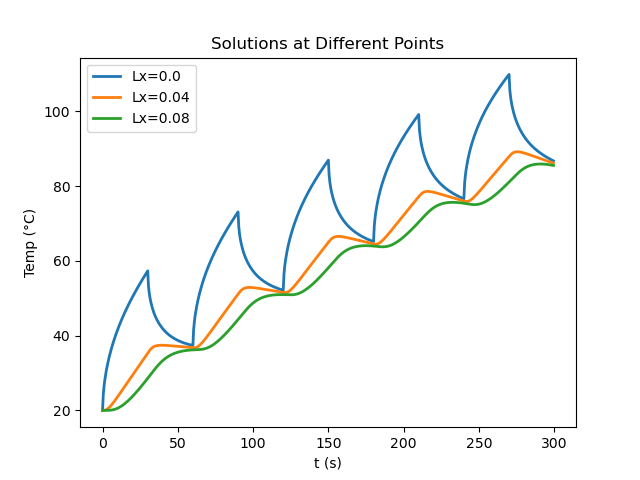
\includegraphics[width=1\linewidth]{images/noFan2.png}
  \caption{}
\end{subfigure}
\caption{Cycling heat flux without fan}
\label{fig:fig}
\end{figure}

\begin{figure}[H]
\begin{subfigure}{.5\textwidth}
  \centering
  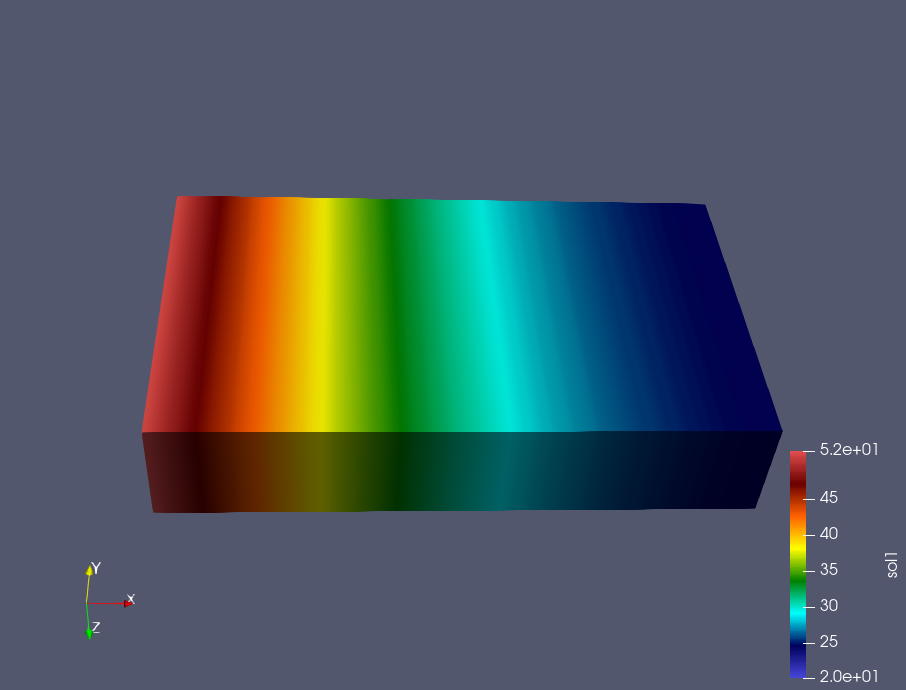
\includegraphics[width=1\linewidth]{images/noFan40s.png}
  \caption{after 20s}
  \label{fig:sfig1}
\end{subfigure}
\begin{subfigure}{.5\textwidth}
  \centering
  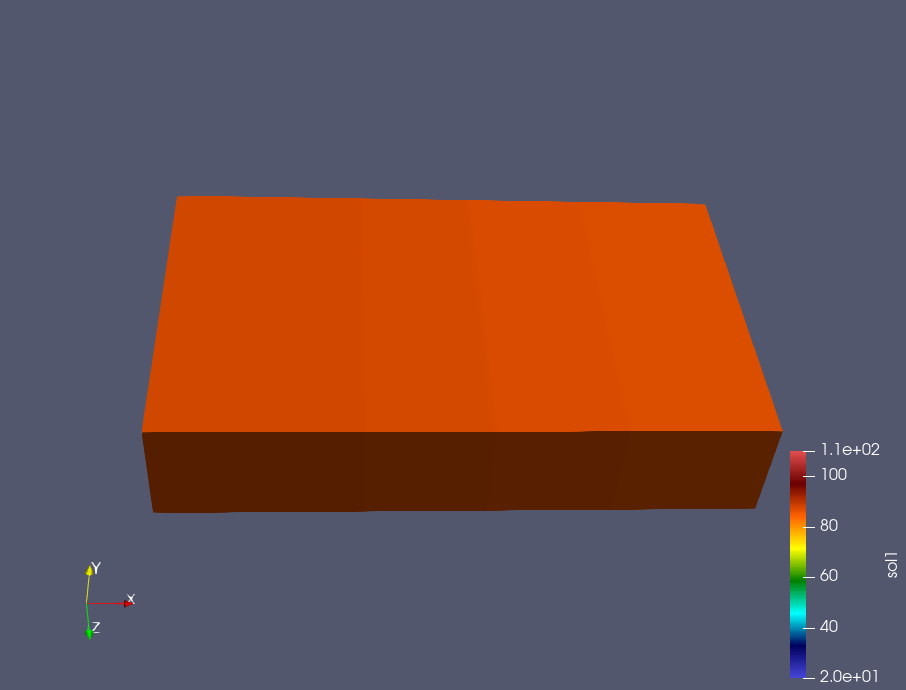
\includegraphics[width=1\linewidth]{images/noFan300s.png}
  \caption{after 300s}
\end{subfigure}
\caption{Cycling heat flux without fan}
\label{fig:fig}
\end{figure}

The temperature definitely goes down when the flux is off but not enough and the heat keeps building up in the material reaching more than 100$\degree$C at the end of our 300s simulation. 

Clearly, even with a cycling heat flux and an 80mm fin, this configuration is not viable. Without an automatic emergency shutdown procedure, the CPU could be irreversibly damaged.

\subsection{Effect of Thermal Conductivity }
Finally let's see what would happen if we could double the thermal conductivity $\kappa$ of the heat fin material going from 164 to 328.

\begin{figure}[H]
\begin{subfigure}{.5\textwidth}
  \centering
  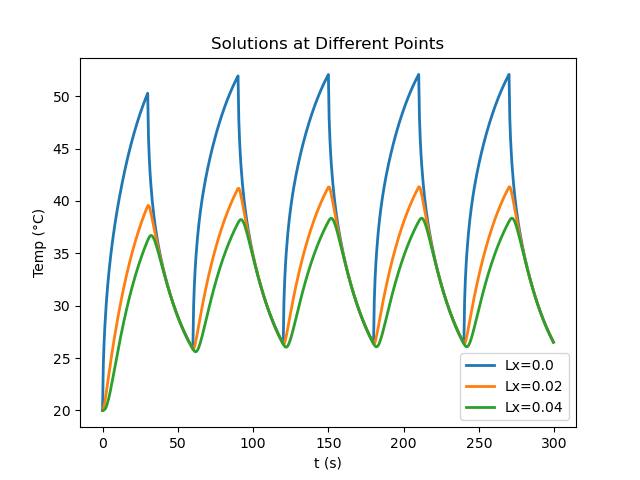
\includegraphics[width=1\linewidth]{images/k164.png}
  \caption{$\kappa=164$}
  \label{fig:sfig1}
\end{subfigure}
\begin{subfigure}{.5\textwidth}
  \centering
  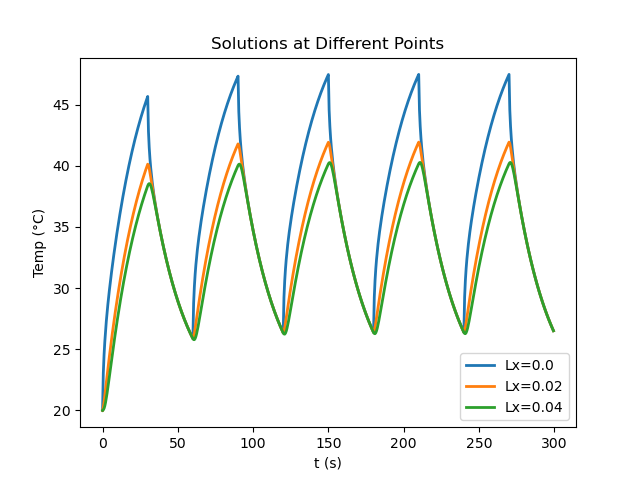
\includegraphics[width=1\linewidth]{images/k328.png}
  \caption{$\kappa=328$}
\end{subfigure}
\caption{Different thermal conductivity}
\label{fig:fig}
\end{figure}

We can notice a difference but not that significant, the fin cool down better and faster but also heat up better and faster. The improvement is probably not worth it for this context of use.

\section{Conclusion}

In this project, we developed a comprehensive simulation framework to analyze the thermal behavior of a single heat fin CPU radiator. The implementation includes a flexible and extensible structure, allowing for the modeling of various heat transfer scenarios.

Our approach involved the creation of a \texttt{Tridiag} template class to handle the banded matrix operations efficiently. The \texttt{Model} base class served as the foundation for specific heat transfer models, with the \texttt{HeatFin} class tailored to the particulars of the problem, including dynamic and stationary simulations.

The \texttt{SolverTime} class provided a systematic way to solve both static and dynamic models, offering options for saving and visualizing results at different time points or spatial locations.

The simulation results demonstrated the impact of various parameters on the temperature distribution within the heat fin. The comparison of different fin lengths, cycling heat flux with and without a fan, and variations in thermal conductivity showcased the versatility of our framework.

Our findings highlighted the significance of fin dimensions, cycling heat flux dynamics, and material properties in determining the effectiveness of the heat fin. The 3D visualizations provided valuable insights into temperature variations over time and space.


\end{document}

